\subsection{Definizione e finalità del Bilancio}
Il \textit{Bilancio d'esercizio} è l'insieme dei documenti contabili che un’impresa deve redigere periodicamente, ai sensi di legge, allo scopo di perseguire il principio di verità ed accertare in modo chiaro, veritiero e corretto la propria situazione patrimoniale e finanziaria, al termine del periodo amministrativo di riferimento, nonché il risultato economico dell'esercizio stesso.

È finalizzato alla misurazione di due grandezze fondamentali:
\begin{itemize}
	\item \textbf{Il Capitale}: prospetto chiamato \textbf{Stato Patrimoniale}
	\item \textbf{Il Reddito\footnote{Reddito = valore prodotti e servizi venduti - valore fattori produttivi impiegati}}: prospetto chiamato \textbf{Conto Economico}
\end{itemize}

\subsection{Forme e finalità del bilancio}
\begin{itemize}
	\item \textbf{GIURIDICA} (imposta dal codice civile) struttura standard per rappresentare la situazione patrimoniale ed economica d’impresa. Finalità:
		\begin{itemize}
			\item Informare sulla consistenza del patrimonio a garanzia di terzi creditori (fornitori, banche, dipendenti, ecc.)
			\item Informare sulla capacità dell’impresa di generare reddito (azionisti, soci/proprietari, ecc.)
		\end{itemize}
	\item \textbf{FISCALE} (imposta dal codice civile). Dichiarazione dei redditi. Il reddito imponibile si ottiene a partire dal bilancio giuridico, operando una serie
		di variazioni (+/-). Finalità:
		\begin{itemize}
			\item Determinare il reddito imponibile (diverso dall’utile pre-imposte = ricavi-costi)
		\end{itemize}
	\item \textbf{GESTIONALE} (non obbligatoria). Si ottiene dal bilancio giuridico (o dai dati di contabilità generale) viene riclassificato e analizzato con opportune tecniche. Finalità:
		\begin{itemize}
			\item reinterpretare il bilancio per ottenere maggiori informazioni sulle caratteristiche gestionali dell’impresa
		\end{itemize}
\end{itemize}

\subsection{Lo Stato Patrimoniale}
Rappresenta la situazione aziendale alla chiusura dell’esercizio: in tale prospetto deve essere evidenziata la situazione \textit{patrimoniale} e \textit{finanziaria} della società che compone l’attivo, quella che compone il passivo e, come differenza tra le due, il patrimonio netto. Lo stato patrimoniale è suddiviso in due sezioni: attivo e passivo.

\textit{Attivo} – Tutti i beni e le proprietà possedute dall’azienda (fabbricati, macchinari, attrezzature) utilizzati per l’esercizio dell’attività, i crediti dell’azienda nei confronti di terzi (clienti, etc.), le disponibilità liquide (cassa, saldi attivi dei conti correnti).

\textit{Passivo} – Debiti dell’azienda verso terzi (fornitori, banche, ...). Il capitale netto indica il debito ideale della società verso i suoi proprietari, ed è costituito dalle riserve e dal capitale sociale.

\begin{table}[H]
	\begin{tabular}{| c | c |}
		\hline
		 Attivo & Passivi e Netto \\
		 \hline
		 Beni e diritti a disposizione & Insieme dei diritti di terzi nei \\
		 dell’impresa per realizzare l’attività &  confronti dell’impresa \\
		 & \\
		 Investimenti in attività & FONTI di finanziamento ricevute \\
		 (IMPIEGHI delle risorse) &  dall’impresa: \\ 
		 & - Passività di terzi \\ 
		 & - Capitale Netto \\
		 \hline
	\end{tabular}
	\centering
	\caption{Schema Stato Patrimoniale}
\end{table}

\begin{figure}[H]
	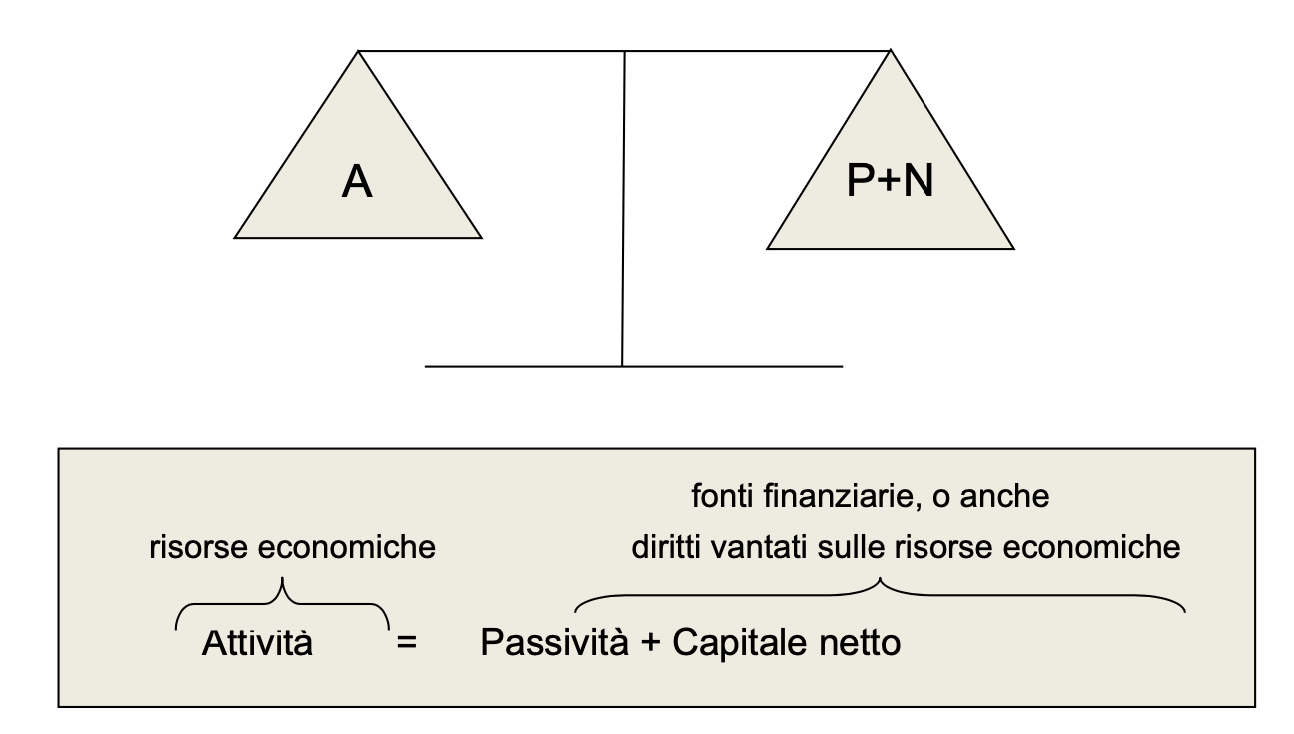
\includegraphics[width=0.8\linewidth]{resources/chapters/Bilancio/images/equazione-bilancio.png}
	\centering
	\caption{Equazione di bilancio}
\end{figure}

\subsubsection{L'attivo}
Le attività di un bilancio includono le attività disponibili di una società, vale a dire quelle merci e altri mezzi con cui la società può lavorare per adempiere i propri compiti operativi. Esse compaiono sul lato sinistro dello stato patrimoniale e comprendono:
\begin{itemize}
	\item crediti verso soci per versamenti ancora dovuti, con separata indicazione della parte già richiamata
	\item immobilizzazioni (immateriali, materiali e finanziarie)
	\item attivo circolante (rimanenze, crediti, attività finanziarie che non costituiscono immobilizzazioni, disponibilità liquide
	\item ratei e risconti
\end{itemize}

\paragraph{Crediti verso i soci}
I crediti verso soci consistono nei versamenti dovuti dai soci per la sottoscrizione di capitale sociale e la copertura di perdite, nonché per eventuali importi connessi (come interessi di conguaglio).

L’espressione “con separata indicazione della parte già richiamata” fa riferimento solamente alle società locatrici che redigono il bilancio secondo l’art. 2423 del Codice Civile. Significa che la parte che è già stata richiesta ai soci, e che quindi è un credito a breve termine, va indicata separatamente.

\paragraph{Immobilizzazioni}
Le immobilizzazioni includono i beni e le attrezzature durevolmente disponibili per la società e utilizzati nelle operazioni commerciali. Per “durevolmente” si intende che se un fattore produttivo verrà venduto a breve, o se una partecipazione verrà dismessa nel prossimo esercizio, non dovrebbe figurare nelle immobilizzazioni. Esse si differenziano in:
\begin{itemize}
	\item Immobilizzazioni immateriali (costi di ricerca e sviluppo, di impianto, brevetti, licenze, ecc.)
	\item Immobilizzazioni materiali (come terreni, fabbricati, attrezzature, macchinari e impianti, mobili, arredi ecc.)
	\item Immobilizzazioni finanziarie (titoli obbligazionari, partecipazioni in altre imprese)
\end{itemize}
Sia per le immobilizzazioni materiali che per quelle immateriali sono previsti gli acconti pagati ai fornitori e le immobilizzazioni vanno iscritte al netto dei fondi di ammortamento, i quali non vanno segnalati nello stato patrimoniale.

\paragraph{Attivo circolante}
I crediti, i titoli e in generale i beni che non hanno la caratteristica di “durevolezza” specificata per la voce delle immobilizzazioni vanno inserite nell’attivo circolante.

Per quanto riguarda i criteri di valutazione vi sono una serie di regole per determinare il valore. Le rimanenze di magazzino, ad esempio, vanno valutate al costo di acquisto o di produzione, oppure nel caso in cui sia minore, al valore di realizzazione (valutabile dall’andamento del mercato).

\paragraph{Ratei e risconti}
I ratei e i risconti attivi rappresentano quote di costi o di proventi comuni ad almeno due esercizi. I ratei si riferiscono ai proventi esigibili negli esercizi successivi mentre i risconti ai costi sostenuti entro la chiusura dell’esercizio anche se di competenza di esercizi successivi.

\subsubsection{Il passivo}
Le passività sono indicate sul lato destro di un bilancio e mostrano da dove provengono le risorse di un’azienda. In generale i fondi di cui l’ente o azienda dispone sono classificate in modo da distinguere i mezzi propri (che confluiscono nel patrimonio netto) da quelli provenienti da terzi. Le passività di un bilancio sono suddivise in:
\begin{itemize}
	\item patrimonio netto (capitale sociale, riserva da sovrapprezzo azioni, riserve di rivalutazione, riserva legale, riserve statutarie, altre riserve (distintamente indicate), riserva per operazioni di copertura dei flussi finanziari attesi, utili (perdite) portati a nuovo, utile (perdita) dell’esercizio, riserva negativa per azioni proprie in portafoglio)
	\item fondo per rischi e oneri
	\item trattamento di fine rapporto
	\item debiti
	\item ratei e risconti
\end{itemize}

\paragraph{Patrimonio netto}
Per patrimonio netto si intendono il capitale sociale sottoscritto dai soci, le riserve, gli utili e le perdite riportati a nuovo, nonché l’utile e la perdita dell’esercizio.

\paragraph{Fondi per rischi ed oneri}
I fondi per rischi ed oneri sono costituiti appunto da fondi destinati a coprire debiti o perdite certe o probabili, il cui ammontare o la cui data di sopravvenienza però non siano ancora noti alla chiusura dell’esercizio

\paragraph{Trattamento di fine rapporto di lavoro subordinato}
Il trattamento di fine rapporto riguarda per l’appunto i debiti contratti nei confronti dei dipendenti per l’indennità di fine rapporto, che saranno sborsati al termine del contratto.

\paragraph{Debiti}
La voce dei debiti è suddivisa in 14 ulteriori sezioni in cui iscrivere i vari tipi di debiti a seconda dell’ente con cui si è contratto il debito (banche, fornitori, ecc.). Occorre iscrivere a ogni voce gli importi esigibili oltre il termine dell’esercizio successivo.

\paragraph{Ratei e risconti}
Anche nella parte passiva del bilancio sono presenti i ratei e i risconti. Mentre però i ratei e risconti attivi si riferivano ai proventi esigibili negli anni successivi e ai costi sostenuti entro la chiusura dell’esercizio, qui al contrario i ratei riguardano i costi esigibili in esercizi successivi (ma di competenza dell’esercizio) e i proventi percepiti entro la chiusura dell’esercizio (ma di competenza di esercizi successivi).

\subsection{Ammortamento}
L'ammortamento è un procedimento amministrativo-contabile con cui il costo di un bene viene ripartito nel corso di più esercizi.

Oggetto del procedimento di ammortamento sono i cosiddetti beni a fecondità ripetuta, ovvero, che mantengono la loro utilità nel corso del tempo, attraverso la procedura di ammortamento, infatti, il costo di tali beni viene spalmato su più anni in ragione della loro durata economica.

La decisione da parte di un’azienda di ripartire il costo di un bene su più anni viene messa in pratica suddividendo il costo del bene in più quote, il cui numero varia in funzione del numero di esercizi in cui il bene (impianto, macchinario etc.) sarà utilizzato.

Ad imporre l’ammortamento è anche il principio contabile della competenza economica delle componenti reddituali, secondo cui non è possibile imputare un bene che viene utilizzato in più esercizi interamente all'esercizio in cui è stato acquistato.
Oggetto dell'ammortamento possono essere:
\begin{itemize}
	\item Le immobilizzazioni materiali ovvero l’insieme di tutti i fattori produttivi ad utilità pluriennale fisicamente tangibili (es. fabbricati, macchinari, impianti, automezzi, attrezzature industriali e commerciali, computer, mobili d'ufficio ecc.)
	\item Le immobilizzazioni immateriali come l’insieme di tutti i fattori produttivi ad utilità pluriennale non fisicamente tangibili (ad esempio, brevetti e marchi, diritti di utilizzo di opere dell'ingegno, concessioni governative, costi di ricerca e sviluppo, costi di pubblicità ecc.)
\end{itemize}
Mentre per le immobilizzazioni materiali viene usato spesso il metodo indiretto, che fa confluire ogni anno la quota nel fondo ammortamento; per le immobilizzazioni immateriali si applica il metodo diretto, consistente nel portare direttamente in deduzione dal costo storico del bene pluriennale le quote d'ammortamento

\begin{itemize}
	\item \textbf{Accantonamento:} A$_i$ = quota annua di ammortamento $\rightarrow$ C.E.
	\item \textbf{Fondo di ammortamento:} $\sum$A$_i$ = somma delle quote accantonate $\rightarrow$ Nota integrativa
	\item \textbf{Valore storico:} V$_0$ = valore di acquisto del bene $\rightarrow$ Nota integrativa
	\item \textbf{Valore netto contabile:} V$_0$ - $\sum$A$_i$ = stima del valore attuale del bene $\rightarrow$ C.E.
\end{itemize}

Alla vendita del bene si hanno i seguenti scenari:
\begin{itemize}
	\item Se Valore di mercato = Valore netto contabile $\rightarrow$ S.P. attivo (Cassa): valore macchinario
	\item Se Valore di mercato > Valore netto contabile $\rightarrow$ C.E. (Plusvalenza=ricavo/provente): V$_m$-V$_{nc}$
	\item Se Valore di mercato < Valore netto contabile $\rightarrow$ C.E. (Minusvalenza=costo): V$_m$-V$_{nc}$
\end{itemize}